%----------------------------------------------------------------------------------------
%	Appendices
%----------------------------------------------------------------------------------------

\graphicspath{ {./parts/} }

\part{Appendices}

\chapter{Gantt Chart}

\begin{figure}[h]
\centering
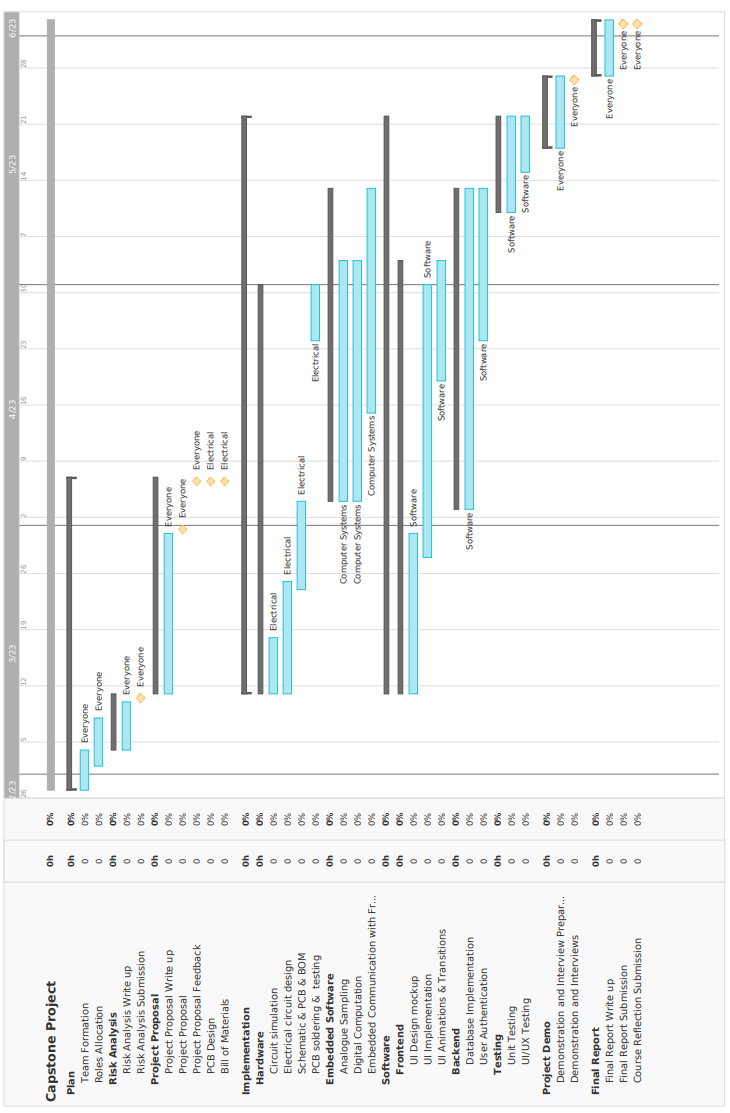
\includegraphics[width=\textwidth]{proposal/parts/Capstone_Project_Gantt_Chart_Hor.png}
\caption{Gantt Chart}
\end{figure}

\chapter{Technical Hardware}

\begin{table}[h]
\centering
\begin{tabular}{|l|m{6cm}|}
    \hline
    Parameter & Value \\
    \hline
    Weight Range & 0 to 3000kg \\
    Wight Accuracy & 0.003kg \\
    Supply Voltage & 6V rechargeable battery \\
    Communication &	RS232 serial communication, optional Bluetooth/WIFI/4-20mA \\
    Weight of load bar	& 11.5kg each \\
    Display & LCD screen \\
    Operating Temperature & -10 to 40°C \\
    \hline
\end{tabular}
\caption{Technical specifiations of AgriEID.}
\label{table:tech specs AgriEID}
\end{table}

\begin{figure}[h]
    \centering
    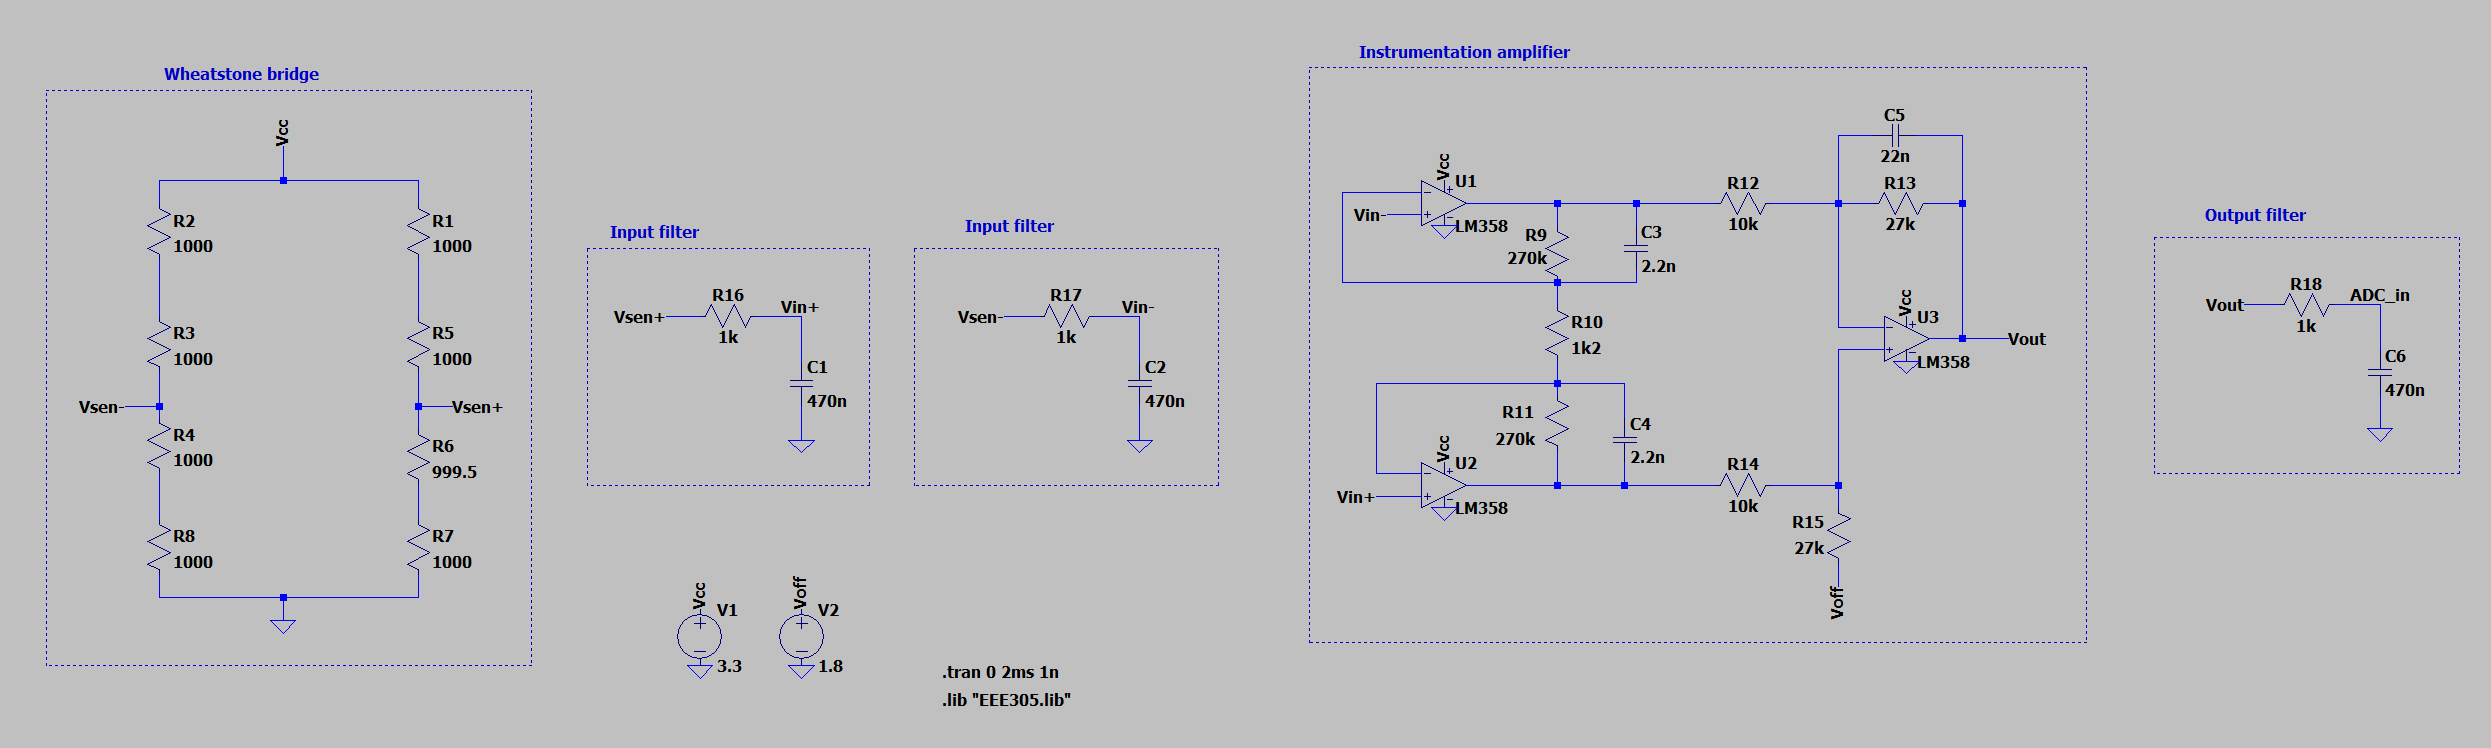
\includegraphics[width=\textwidth]{proposal/parts/hardware-circuit.png}
    \caption{Hardware design divided into functional blocks.}
    \label{fig:hardware}
\end{figure}


\begin{table}[h]
\begin{center}
\begin{tabular}{|l|l|}
    \hline
    Parameter & Value \\
    \hline
    Weight Range & 0 to 25kg \\
    Weight Accuracy & 0.25kg \\
    Supply Voltage & 4 x AAA Batteries \\
    Output Voltage Range & 0.2 to 1.89V \\
    Operating Temperature & 0 to 40°C \\
    Display & LED indicates a successful reading \\
    Compliance & RoHS and WEEE (AS/NZS 5377) \\
    \hline
\end{tabular}
\caption{Technical specifications of the proposed design.}
\label{table:tech specs}
\end{center}
\end{table}

\begin{table}[h]
    \begin{center}
    \begin{tabular}{|l|l|}
        \hline
        Voltage input & Voltage output \\
        \hline
        0mV & 1.799V \\
        -0.206mV & 1.549V \\
        -0.412mV & 1.299V \\
        -0.619mV & 1.043V \\
        -0.825mV & 0.799V \\
        -1.032mV & 0.549V \\
        -1.238mV & 0.299V \\
        \hline
    \end{tabular}
    \caption{Simulation results.}
    \label{table:simulation}
    \end{center}
\end{table}



\chapter{Simulation results from LTspice}


\begin{figure}[h]
\centering
\includegraphics[width=\textwidth]{proposal/parts/0mV.png}
\caption{0mV input.}
\end{figure}

\begin{figure}[h]
\centering
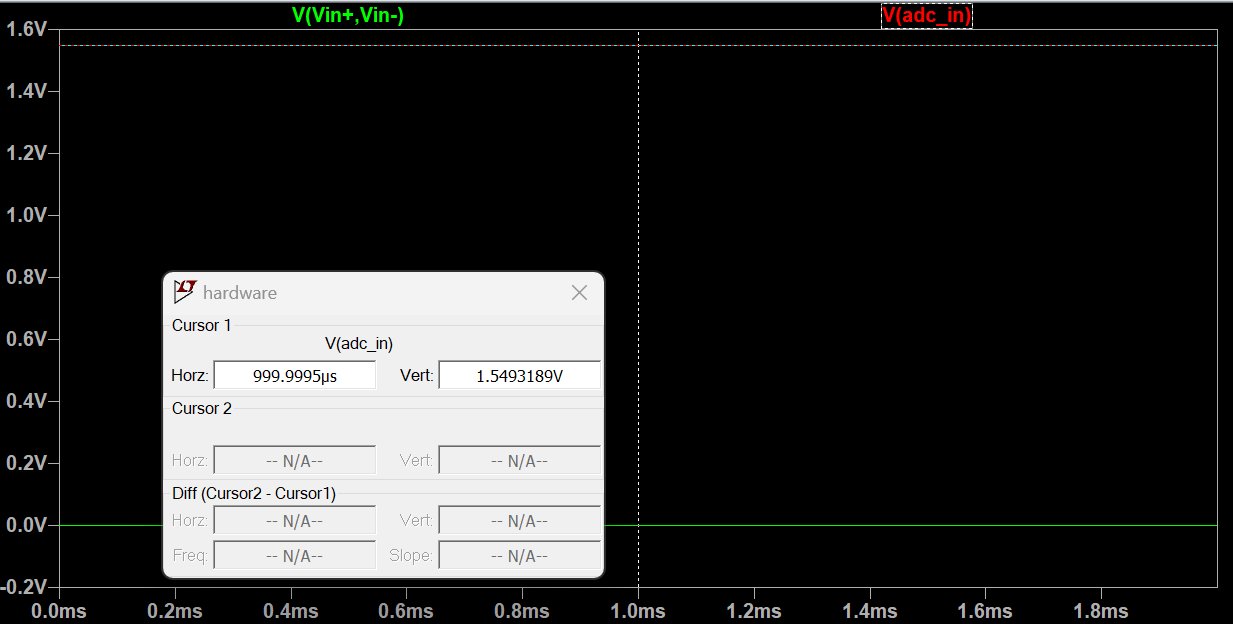
\includegraphics[width=\textwidth]{proposal/parts/-0.206mV.png}
\caption{-0.206mV input.}
\end{figure}

\begin{figure}[h]
\centering
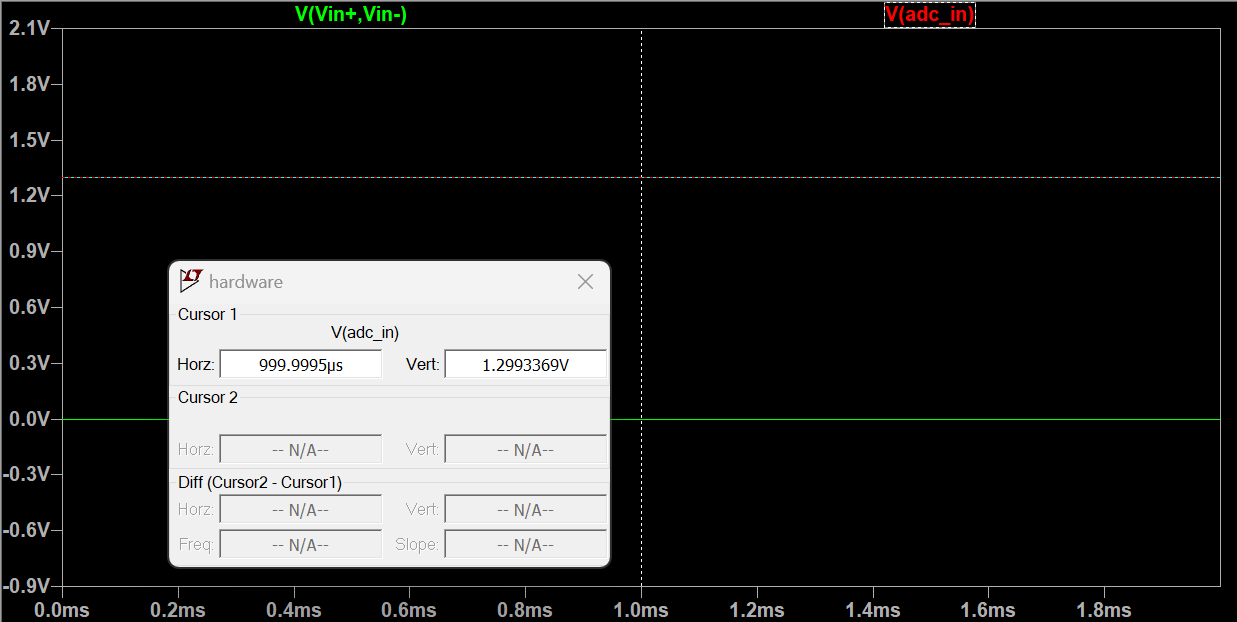
\includegraphics[width=\textwidth]{proposal/parts/-0.412mV.png}
\caption{-0.412mV input.}
\end{figure}

\begin{figure}[h]
\centering
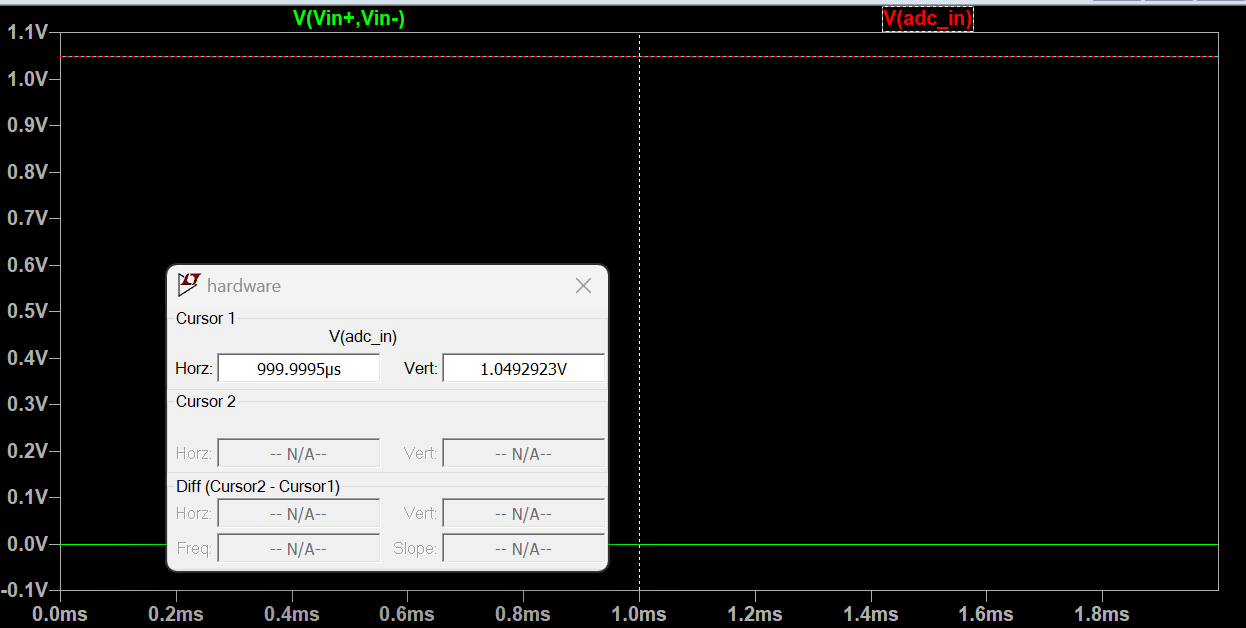
\includegraphics[width=\textwidth]{proposal/parts/-0.619mV.png}
\caption{-0.619mV input.}
\end{figure}

\begin{figure}[h]
\centering
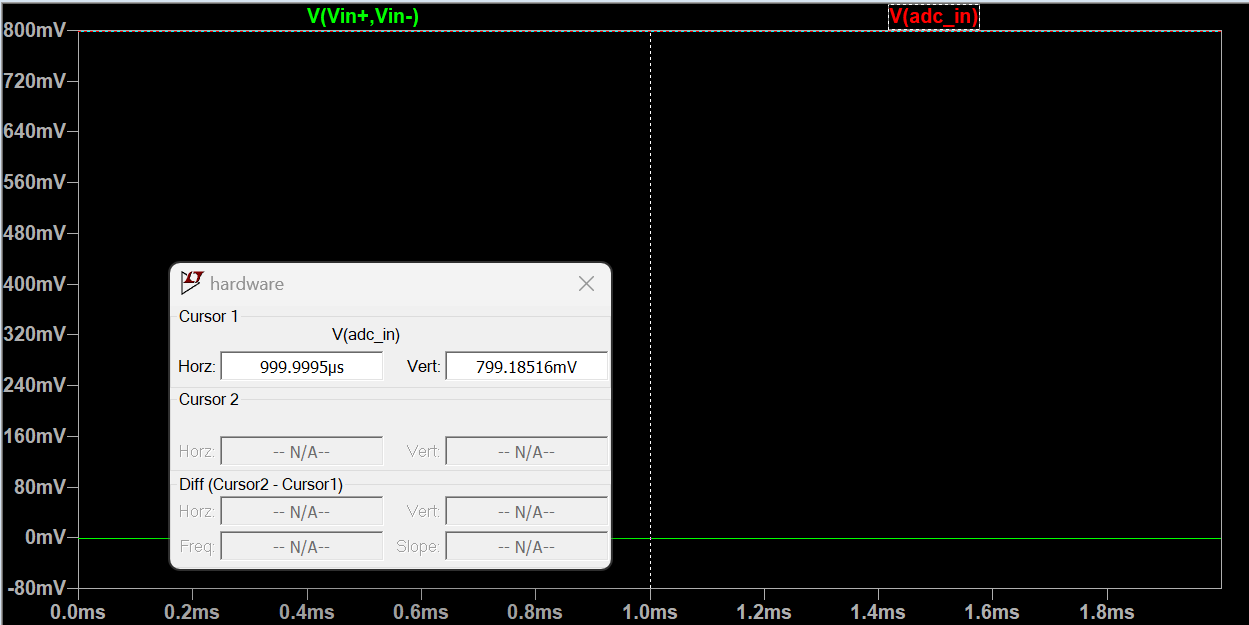
\includegraphics[width=\textwidth]{proposal/parts/-0.825mV.png}
\caption{-0.825mV input.}
\end{figure}

\begin{figure}[h]
\centering
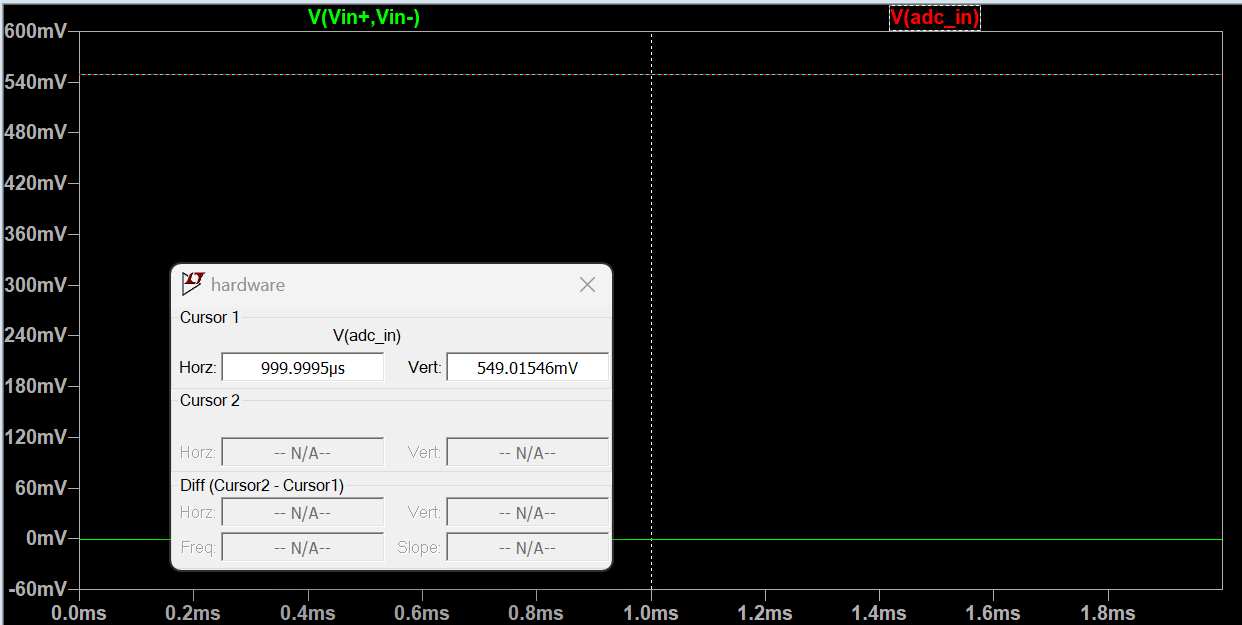
\includegraphics[width=\textwidth]{proposal/parts/-1.032mV.png}
\caption{-1.032mV input.}
\end{figure}

\begin{figure}[h]
\centering
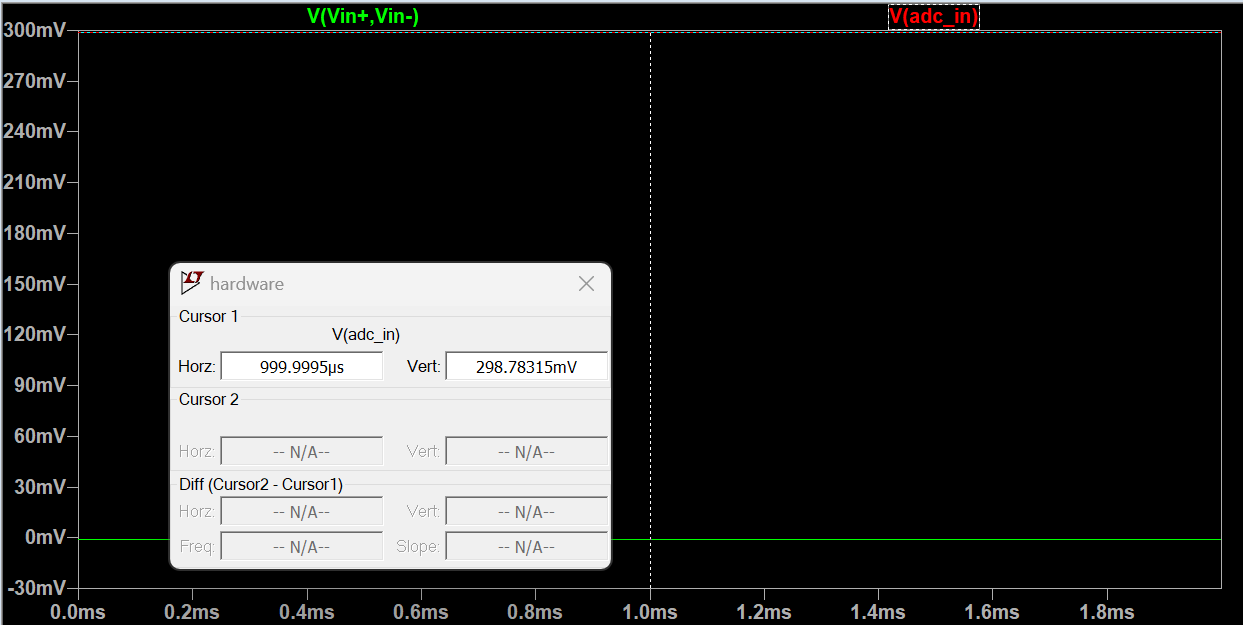
\includegraphics[width=\textwidth]{proposal/parts/-1.238mV.png}
\caption{-1.238mV input.}
\end{figure}

\chapter{Bill of Materials}

\begin{figure}[h]
\centering
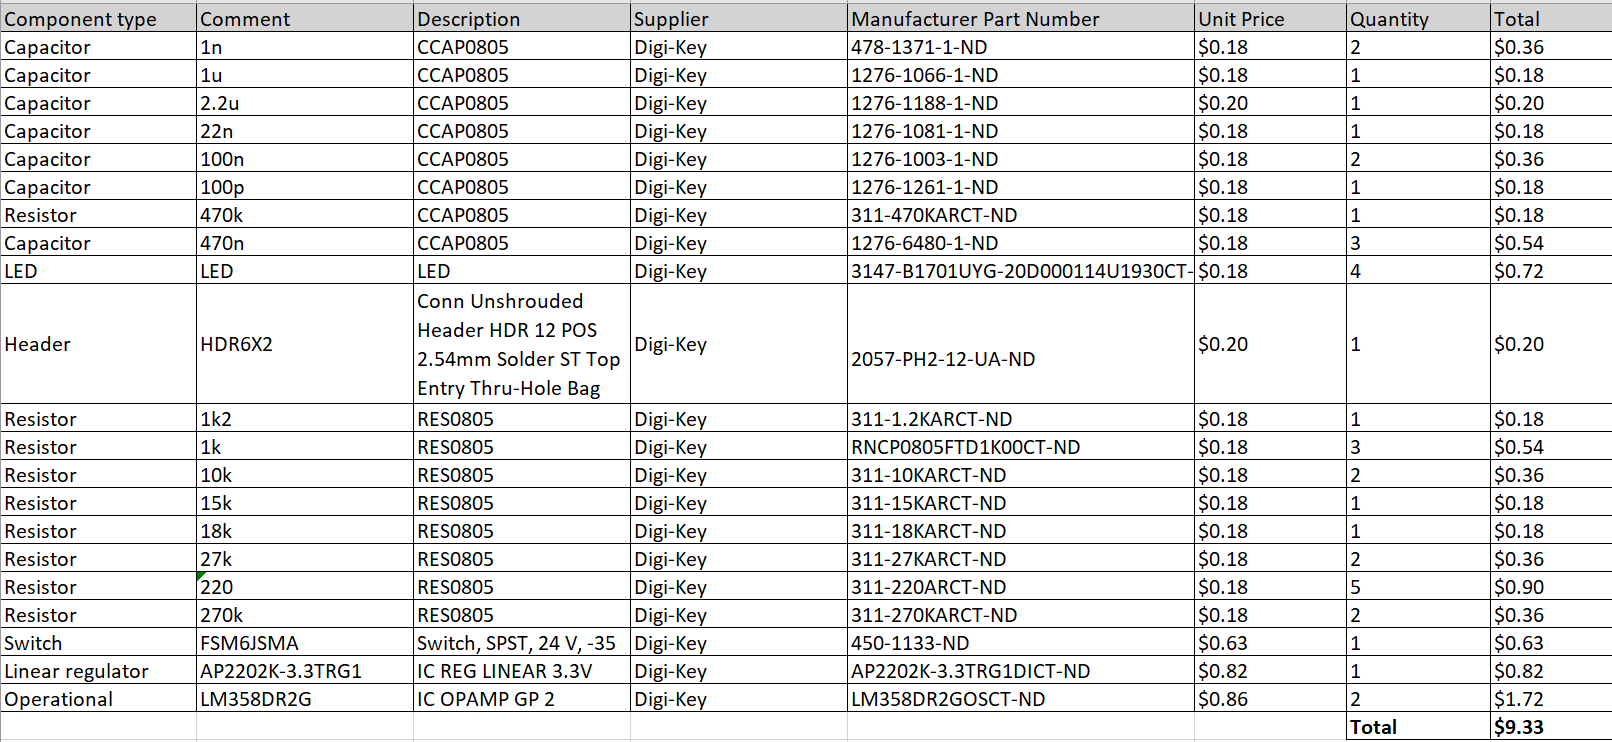
\includegraphics[width=\textwidth]{proposal/parts/BOM.png}
\caption{Bill of Materials}
\end{figure}

\chapter{Database Design}

\begin{figure}[h]
\centering
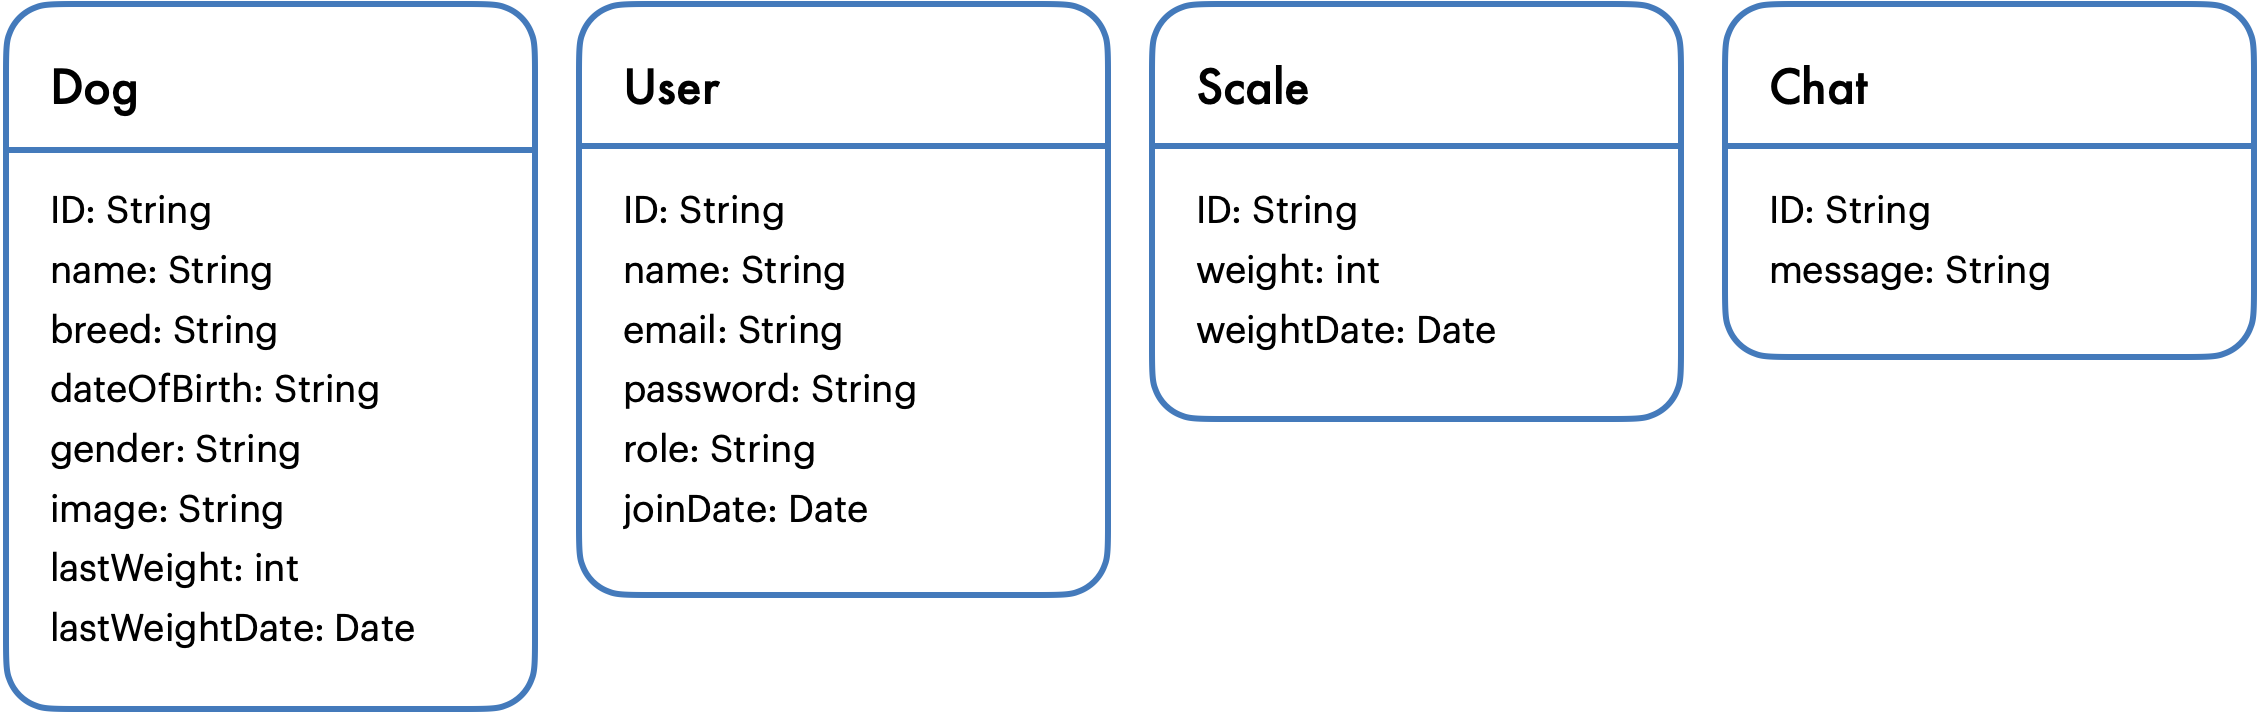
\includegraphics[width=\textwidth]{proposal/parts/database.png}
\caption{Database Design}
\label{figure:database}
\end{figure}

\chapter{Web Platform}

\begin{figure}[h]
\centering

\includegraphics[width=\textwidth]{proposal/parts/login.png}
\caption{Login Page}
\label{figure:login}
\end{figure}

\begin{figure}[h]
\centering
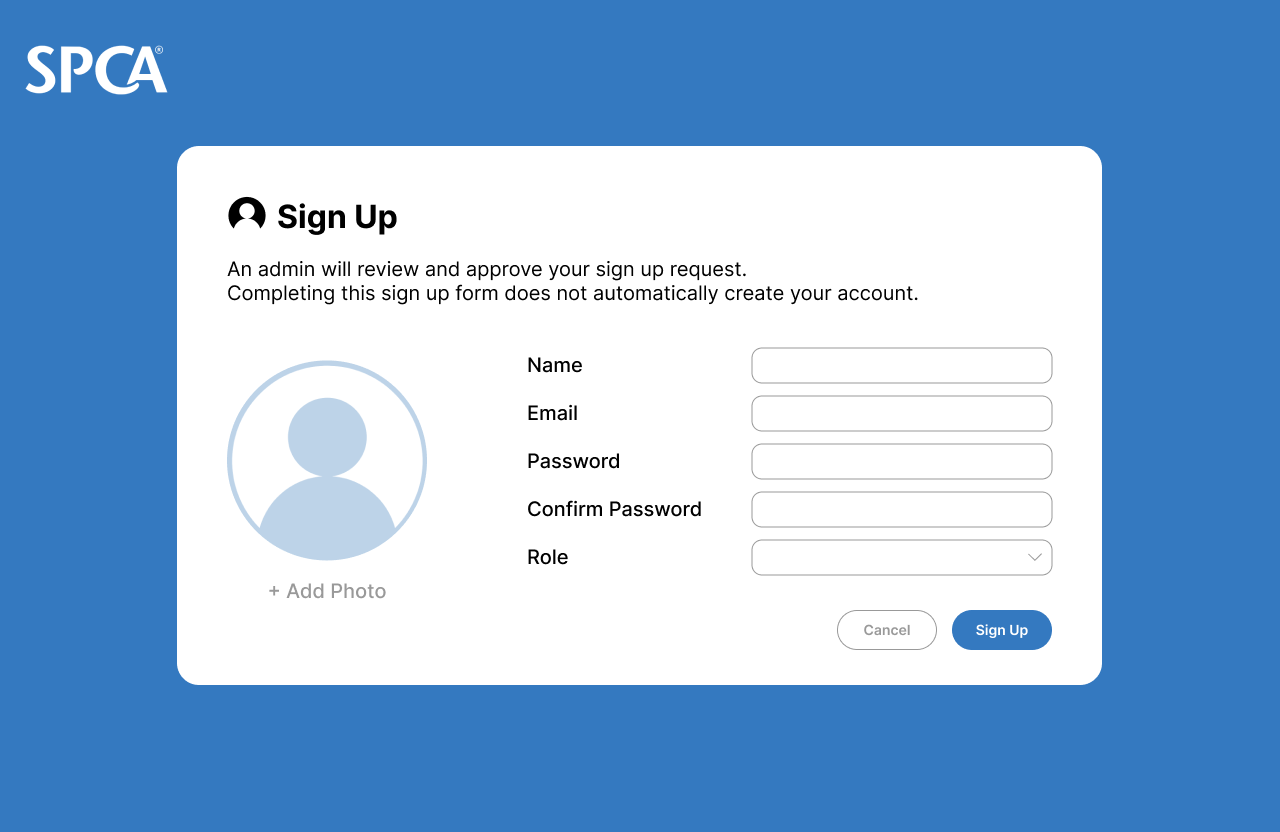
\includegraphics[width=\textwidth]{proposal/parts/sign-up.png}
\caption{Sign Up Page}
\label{figure:sign up}
\end{figure}

\begin{figure}[h]
\centering

\includegraphics[width=\textwidth]{proposal/parts/sign-up-confirm.png}
\caption{Sign Up Confirmation Message}
\label{figure:sign up message}
\end{figure}

\begin{figure}[h]
\centering
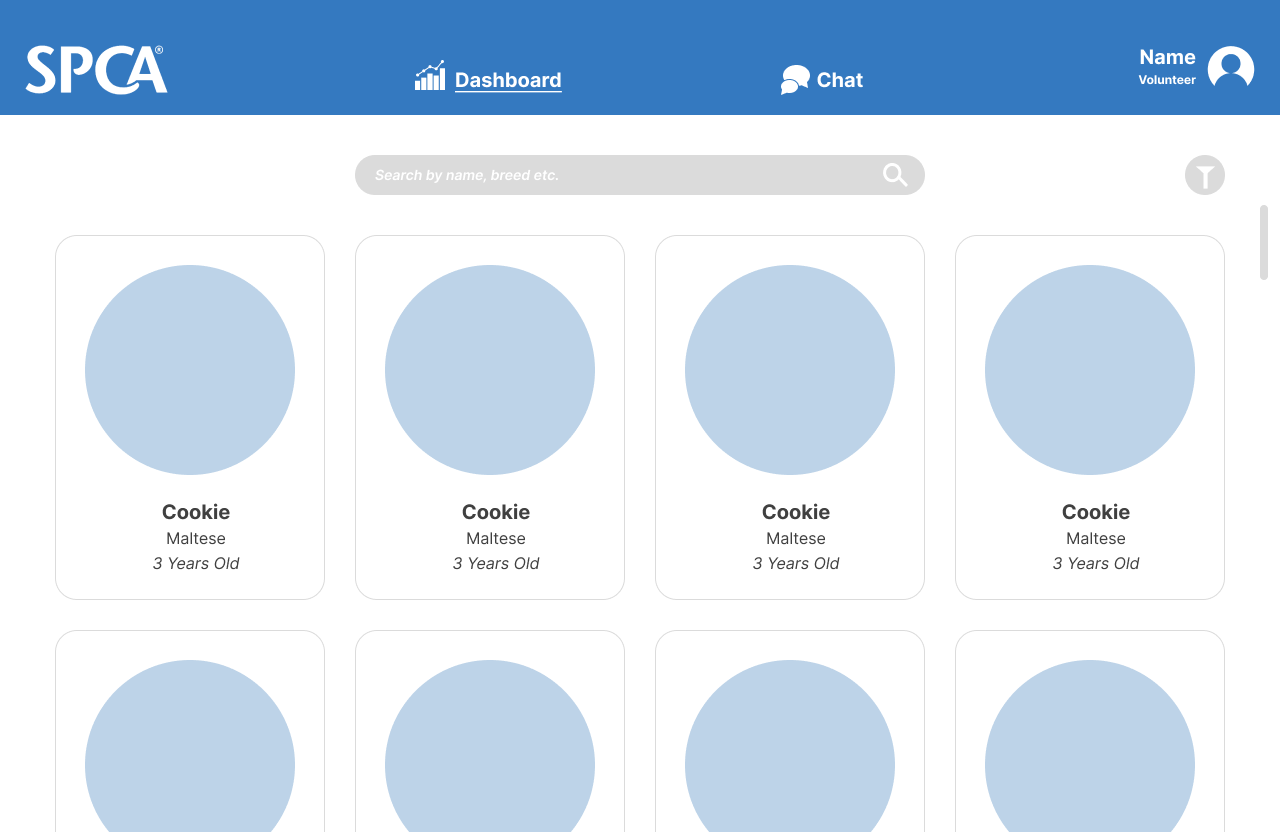
\includegraphics[width=\textwidth]{proposal/parts/dashboard.png}
\caption{Dashboard}
\label{figure:dashboard}
\end{figure}

\begin{figure}[h]
\centering
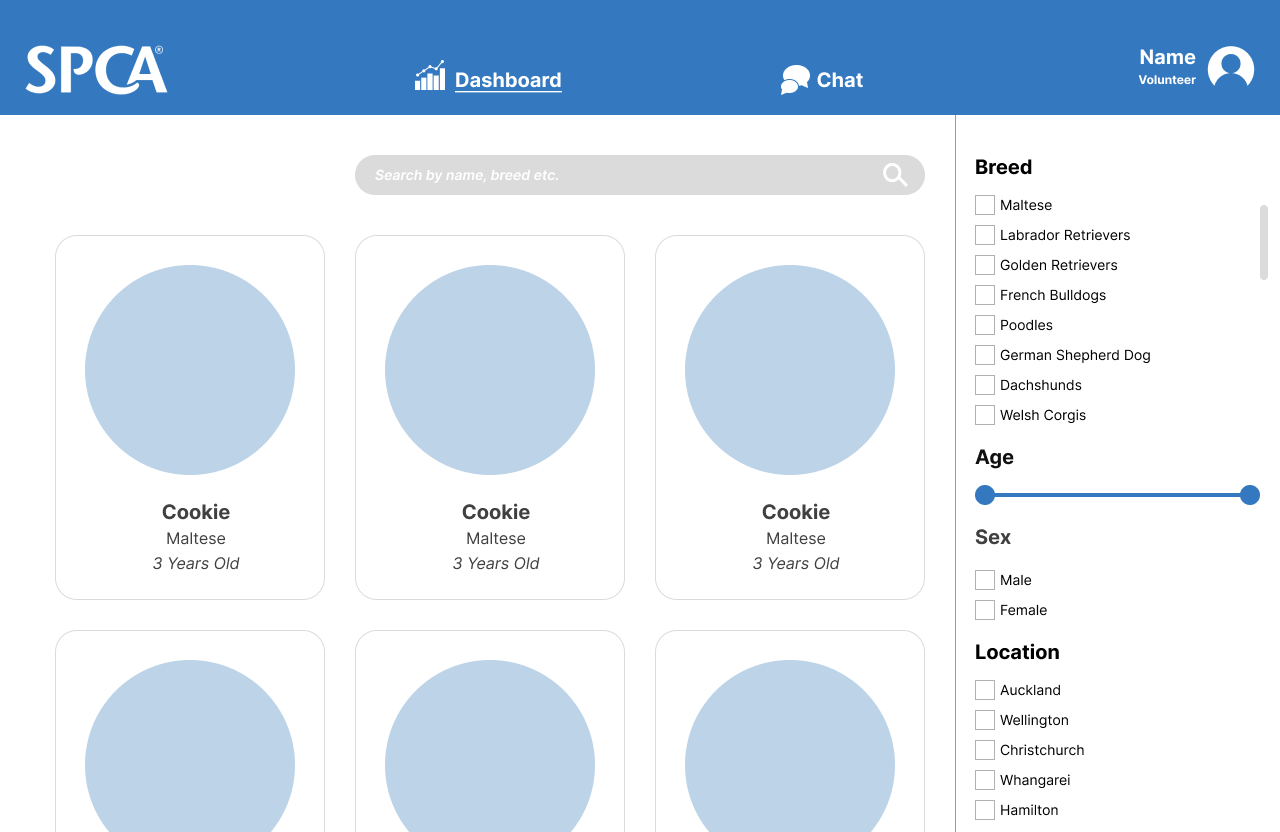
\includegraphics[width=\textwidth]{proposal/parts/dashboard-filter.png}
\caption{Dashboard Filter}
\label{figure:dashboard filter}
\end{figure}

\begin{figure}[h]
\centering
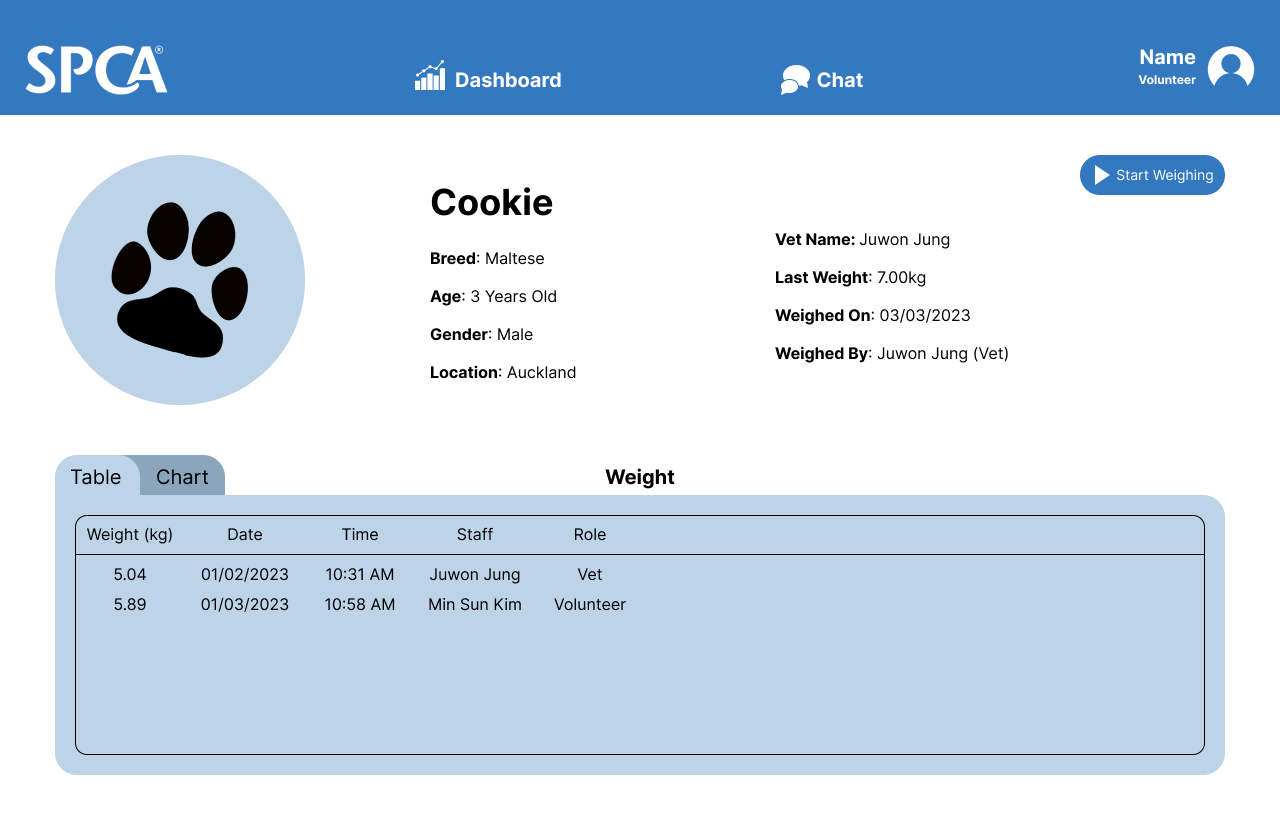
\includegraphics[width=\textwidth]{proposal/parts/dashboard-dog-detail-table.png}
\caption{Dog Detail View - Table}
\label{figure:dog detail table}
\end{figure}

\begin{figure}[h]
\centering
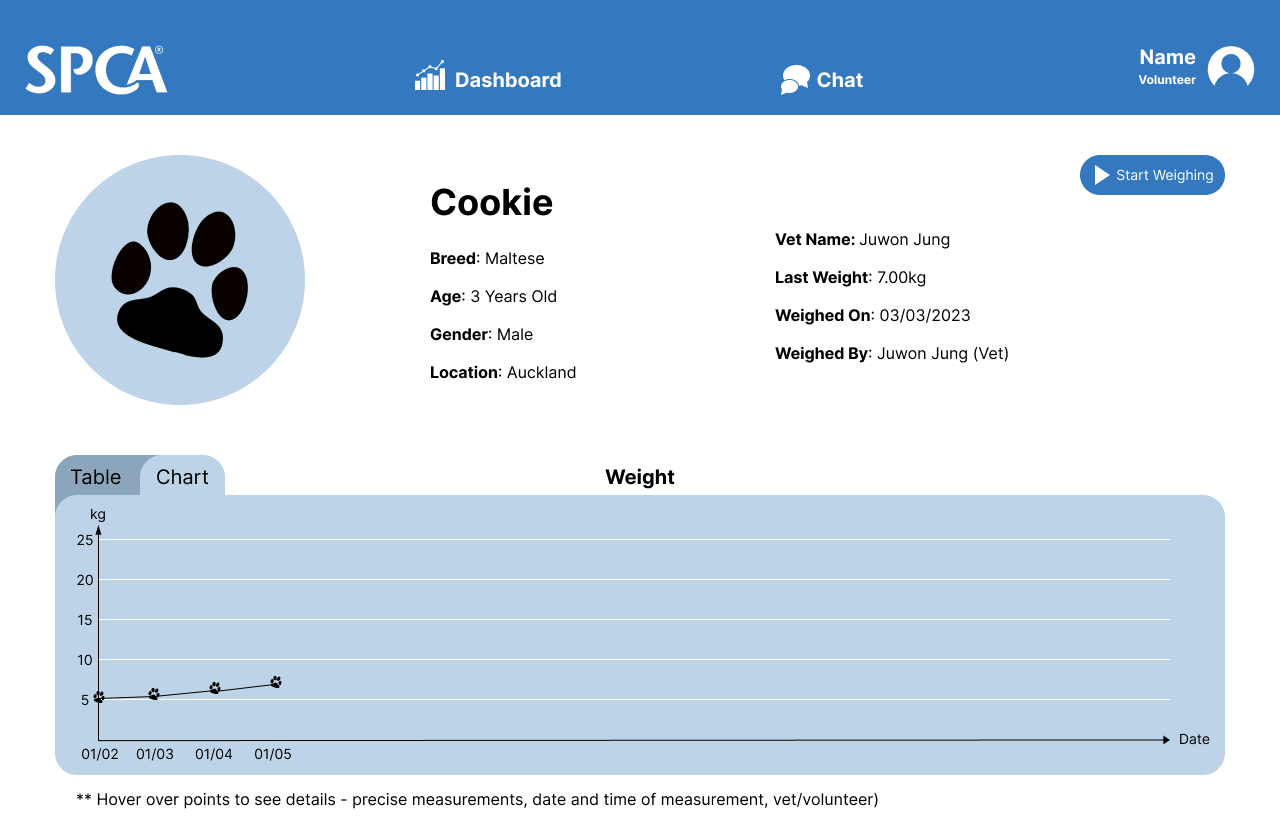
\includegraphics[width=\textwidth]{proposal/parts/dashboard-dog-detail-graph.png}
\caption{Dog Detail View - Graph}
\label{figure:dog detail graph}
\end{figure}

\begin{figure}[h]
\centering
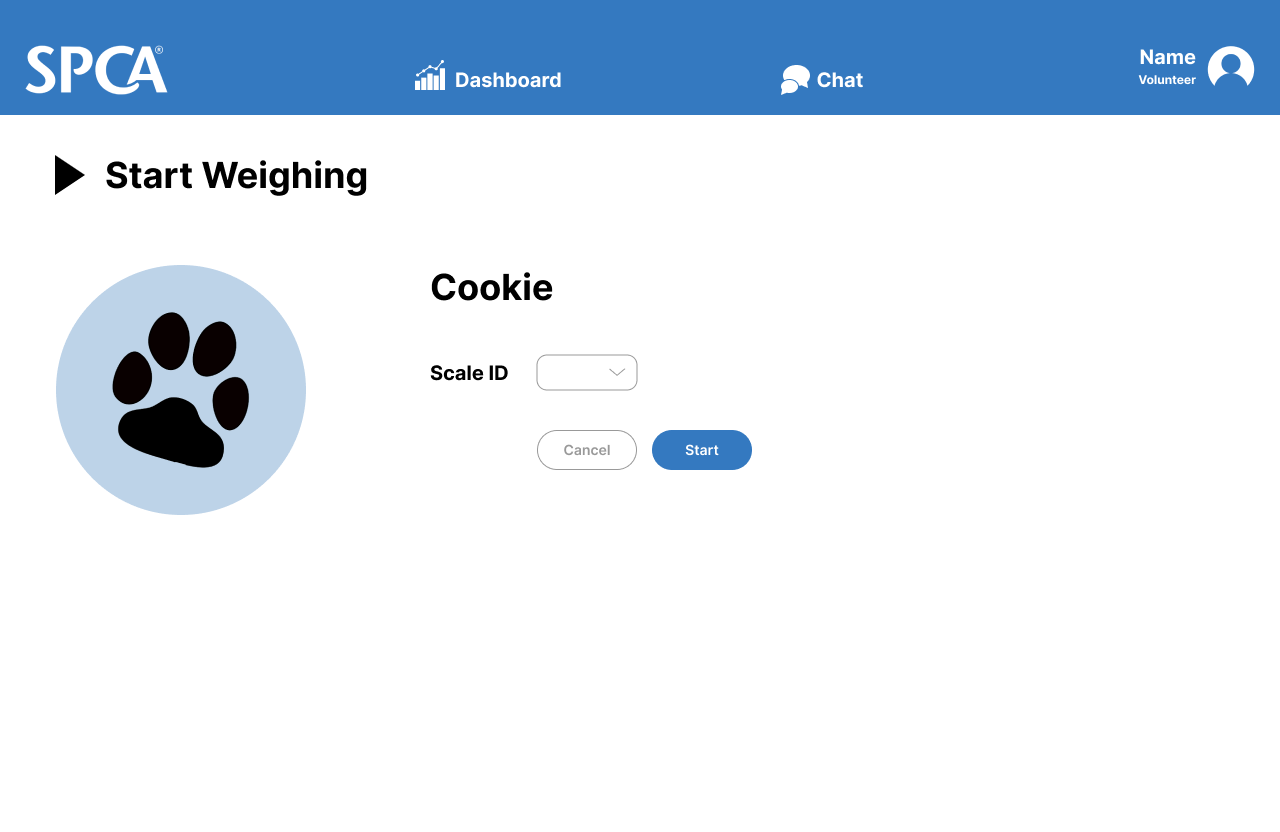
\includegraphics[width=\textwidth]{proposal/parts/add-data-1.png}
\caption{Start Weighing - Select Scale ID}
\label{figure:add data 1}
\end{figure}

\begin{figure}[h]
\centering
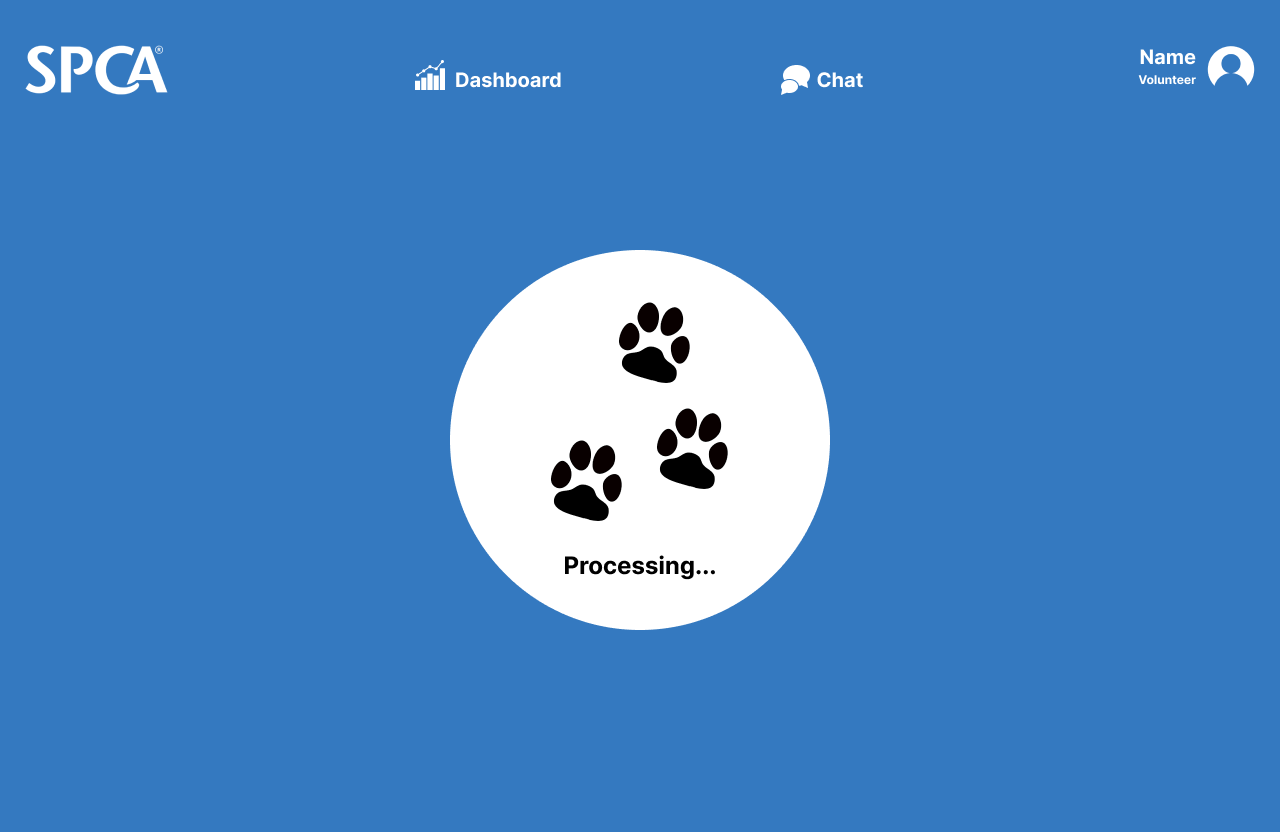
\includegraphics[width=\textwidth]{proposal/parts/add-data-2.png}
\caption{Start Weighing - Processing Data}
\label{figure:add data 2}
\end{figure}

\begin{figure}[h]
\centering
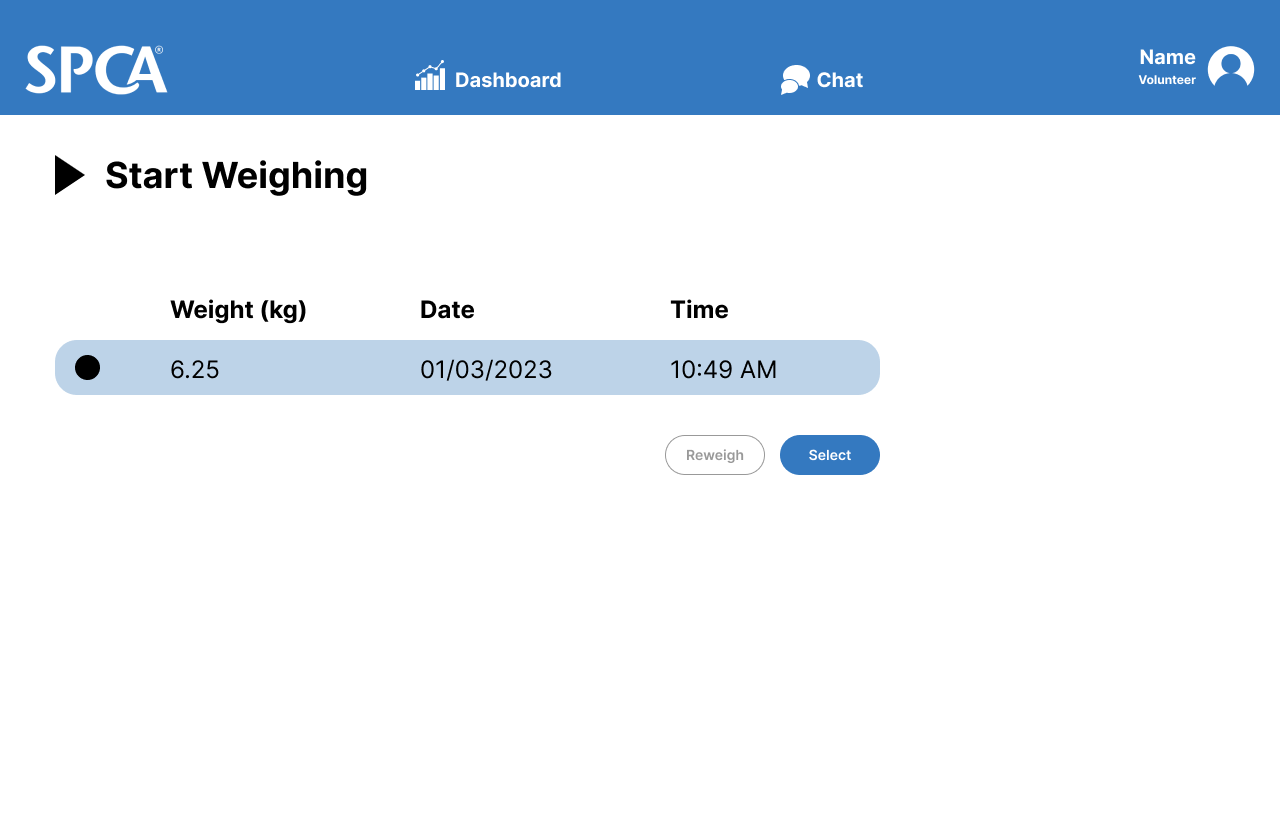
\includegraphics[width=\textwidth]{proposal/parts/add-data-3.png}
\caption{Start Weighing - Select Data}
\label{figure:add data 3}
\end{figure}

\begin{figure}[h]
\centering
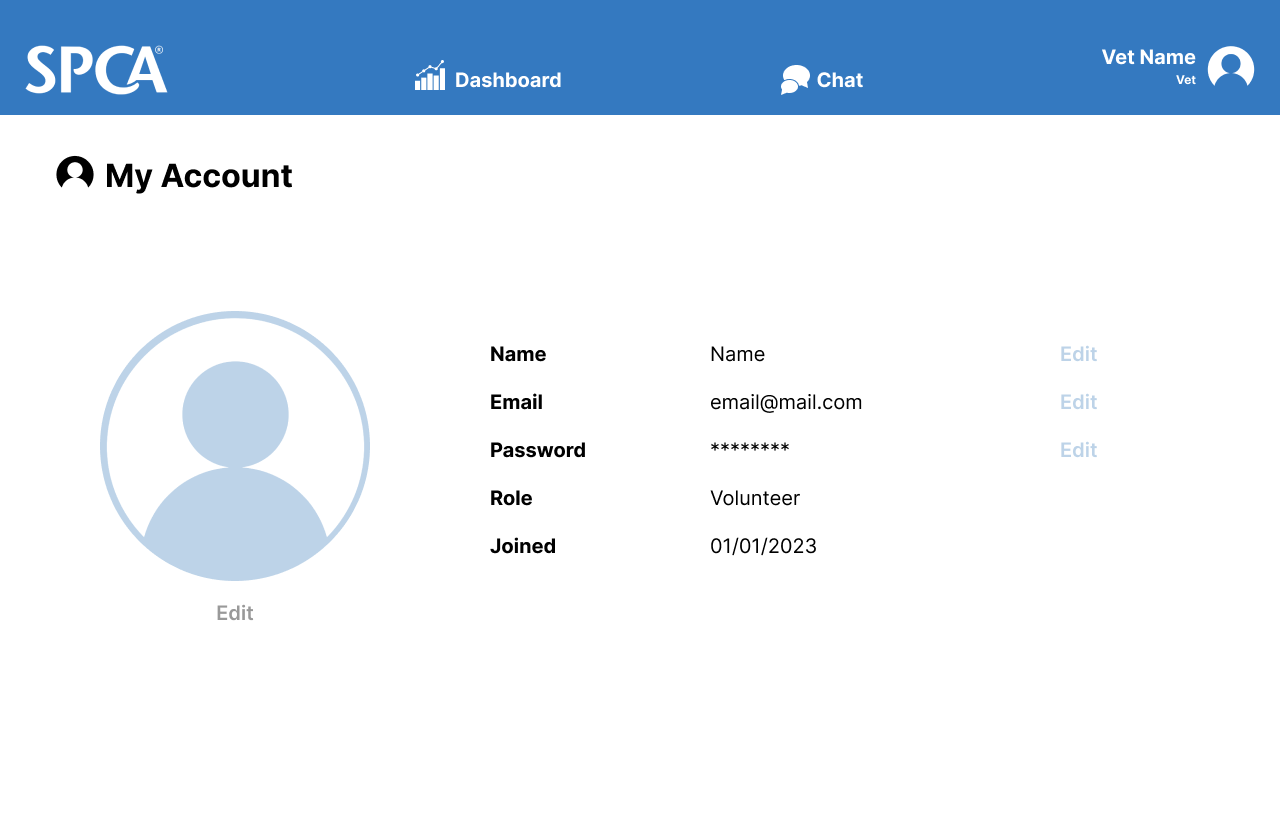
\includegraphics[width=\textwidth]{proposal/parts/my-account.png}
\caption{My Account}
\label{figure:account}
\end{figure}

\begin{figure}[h]
\centering
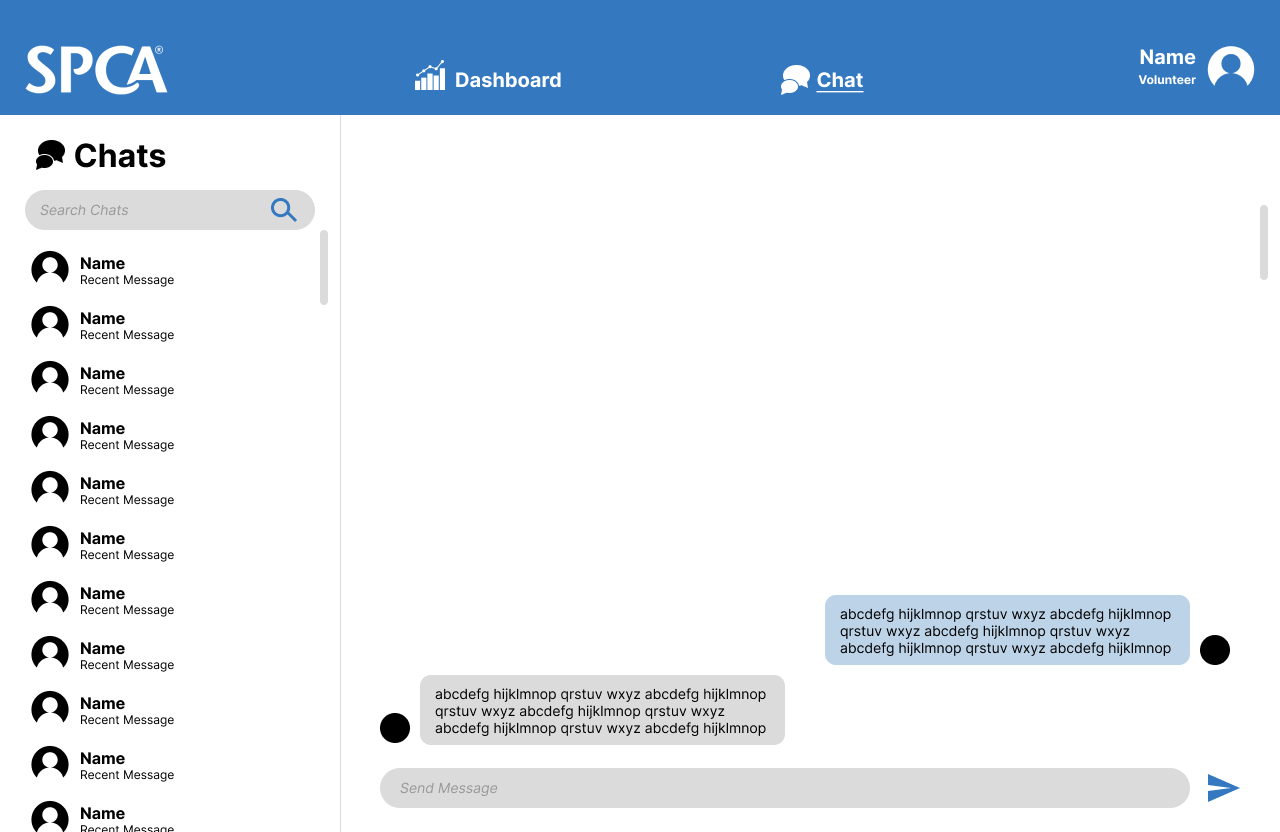
\includegraphics[width=\textwidth]{proposal/parts/chat.png}
\caption{Chat}
\label{figure: chat}
\end{figure}

\begin{figure}[h]
\centering
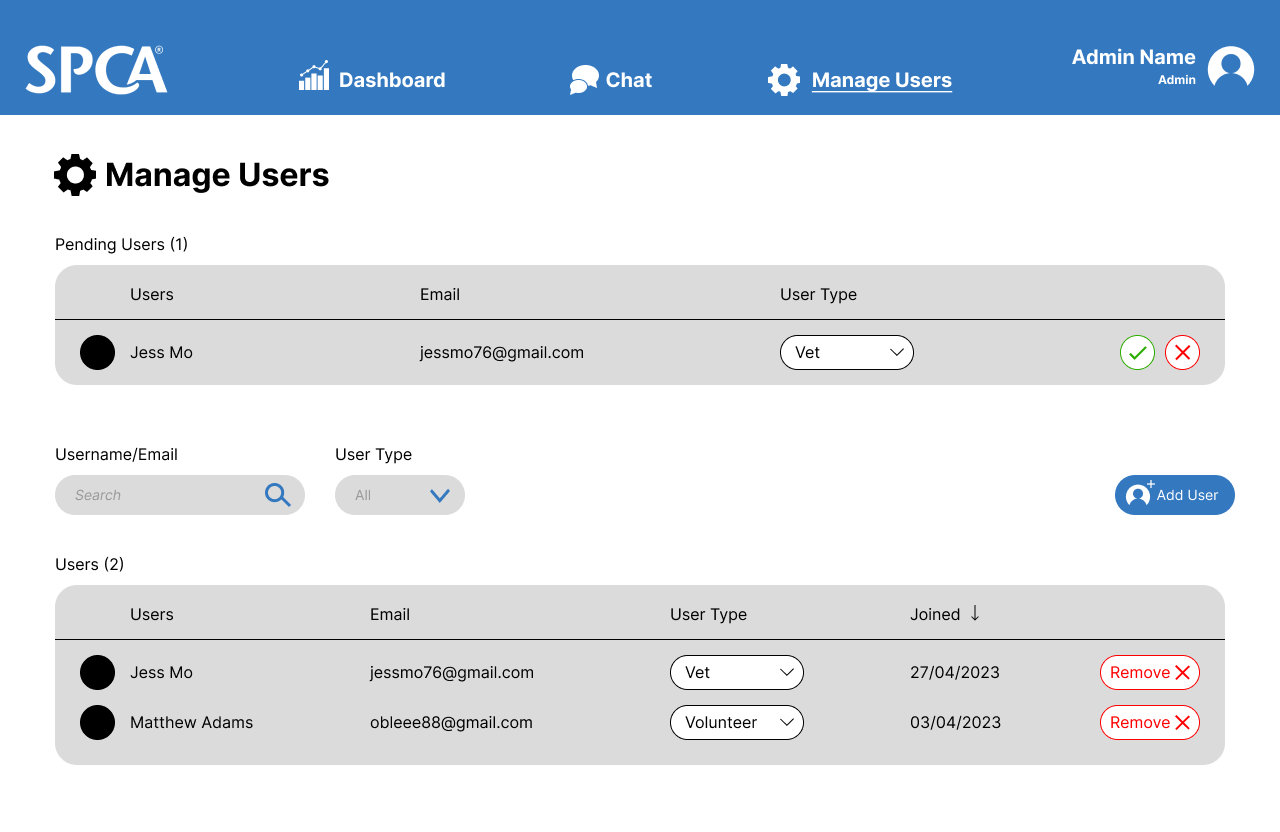
\includegraphics[width=\textwidth]{proposal/parts/admin-manage-users.png}
\caption{Manage Users (Admin View)}
\label{figure:manage users}
\end{figure}

\begin{figure}[h]
\centering
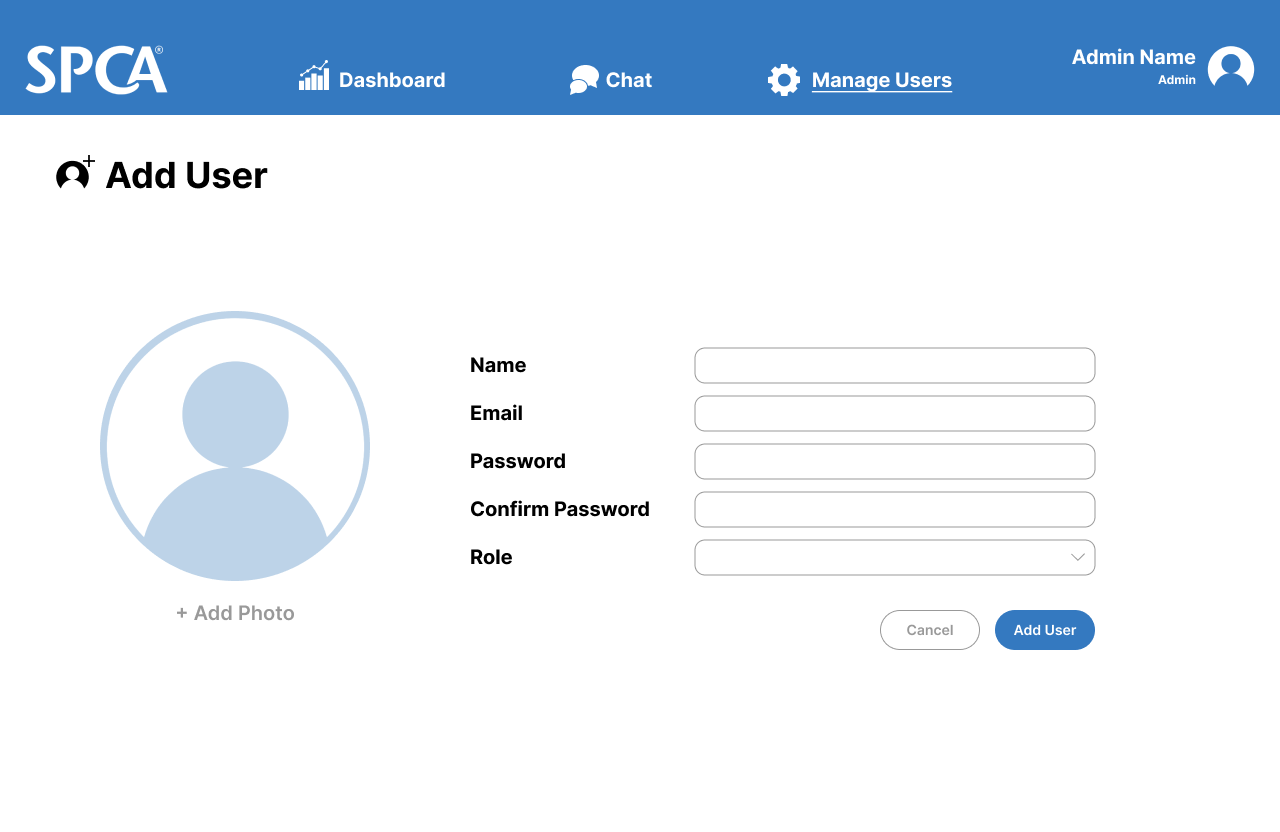
\includegraphics[width=\textwidth]{proposal/parts/admin-add-user.png}
\caption{Add User (Admin View)}
\label{figure:add user}
\end{figure}


